\section{Exploratory data analysis}\label{EDA}

Exploratory data analysis (EDA) is a process in which we familiarise ourselves with data \parencite{tukey1977exploratory}. Listed in the tree structure bellow are the files originally provided to us. Listed bellow can be seen split sections, based on the nested paths (chat, combined and flamingo data).

\dirtree{%
.1 DataSet.
.2 dataset\_attribute\_desc.doc.
.3 description of the dataset.
.2 combined-data.csv.
.2 chat-data.
.3 chat\_join\_team\_chat.csv.
.4 When a user joins a team, a new record is going to be added to this file. 
.3 chat\_leave\_team\_chat.csv.
.4 When a user leaves a team, a new record is going to be added to this file. 
.3 chat\_mention\_team\_chat.csv.
.4 When a user gets a mention, a new record is going to be added to this file. 
.3 chat\_respond\_team\_chat.csv.
.4 When a player with chatid2 responds to a post by another player with chatid2, a new line is added in this file.
.2 flamingo-data.
.3 ad-clicks.csv.
.4 Database of clicks on ads.
.3 buy-clicks.csv.
.4 Database of purchases.
.3 game-clicks.csv.
.4 A record of each click a user performed during the game.
.3 level-events.csv.
.4 A record of each level event for a teams,lLevel events are recorded when a team ends or begins a new level.
.3 team-assignments.csv.
.4 A record of each time a user joins a team.
.3 team.csv.
.4 A record of each team in the game.
.3 user-session.csv.
.4 A record of each session a user plays.
.3 users.csv.
.4 Database of the game users.
}

Originally the following items were zipped:
\begin{itemize}
    \item chat-data.zip
    \item combined-data.zip
    \item flamingo-data.zip
\end{itemize}


\subsection{Combined data}\label{EDA}

This is a general representation of data. It combines different items from flamingo data together into one.
\begin{center}
\begin{longtable}{ |l|l| } 
 \hline
 Attribute & Description\\ 
 \hline
 userId & id of the user\\ 
 \hline
 userSessionId & id of the session\\ 
 \hline
 teamLevel & level team is at\\ 
 \hline
 platformType & what platform user is on\\ 
 \hline
 count\_gameclicks & number of game clicks\\ 
 \hline
 count\_hits & number of hits\\ 
 \hline
 count\_buyId & id of buy\\ 
 \hline
 avg\_price & average buy price\\ 
 \hline

\caption{combined-data.csv}
\end{longtable}
\end{center}

Discovering missing data showcases two things; missing data in count\_buyId and avg\_price and correlation between them. It seems like attributes are coupled together since user who buys a product gets buy ID and average price of it. Based on that logic, if item is not bought there is no ID and no price. Situation like this could be avoided by having product with id 0 and price 0 inside. This would help us expose actual missing values since at the moment we cannot confirm if missing values are intentional or by mistake.

\begin{figure}[H]
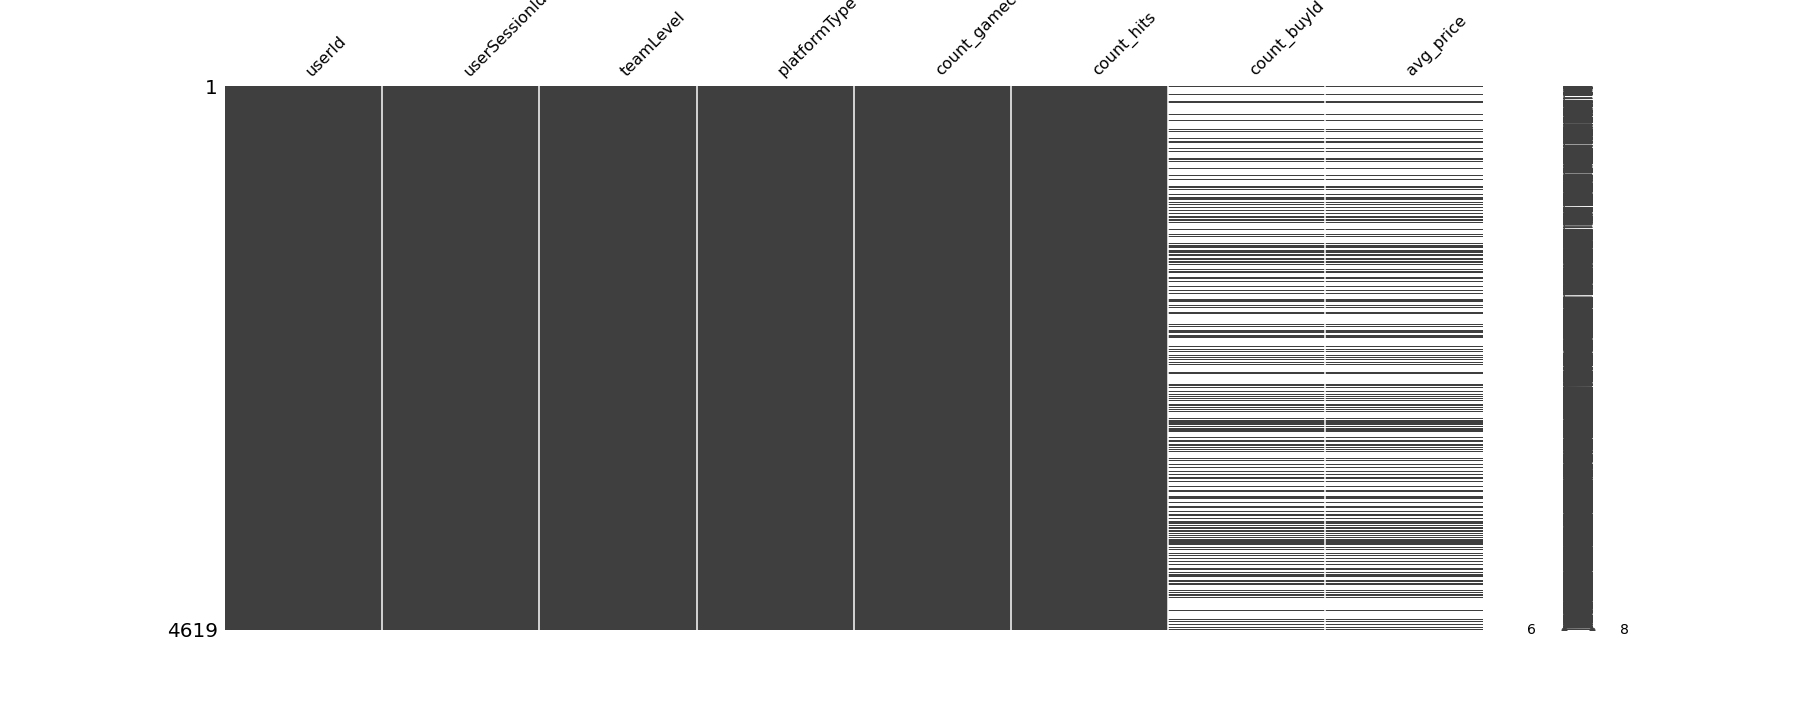
\includegraphics[scale=0.25]{img/Graphs/combinedData/missingno_combinedData.png}
\centering
\caption{combinedData\_msno}
\label{fig:combinedData_msno}
\end{figure}


Knowing our audience is key thing, therefore we need to know what platform is the most used for the game. Pie chart bellow showcases that mobile platform (mainly iphone) is what majority of our players use.
\begin{figure}[H]
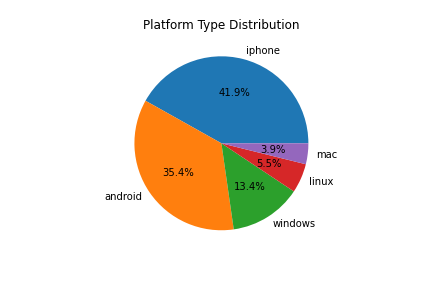
\includegraphics[scale=0.85]{img/Graphs/combinedData/correlationPlot_combinedData.png}
\centering
\caption{combinedData\_correlationPlot}
\label{fig:combinedData_correlationPlot}
\end{figure}

To understand skills, we can compare platforms between each other. Although iphone has the most game clicks (due to being the most popular) and the most hits, android seems to be fairly close to iphone. That could suggest that android players are getting more hits either due to skill or due to platform advantage.
\begin{figure}[H]
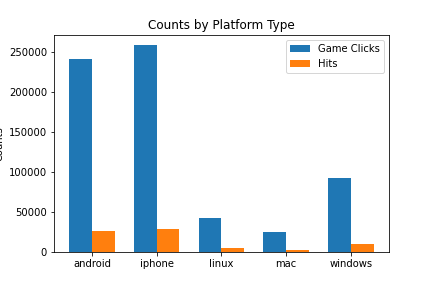
\includegraphics[scale=0.85]{img/Graphs/combinedData/multiGrap_combinedData.png}
\centering
\caption{combinedData\_multiGrap}
\label{fig:combinedData_multiGrap}
\end{figure}

Spending habits can tell us a lot about the user. By averaging price spent per platform we can see that iphone users spend the most, but what is surprising is mac users. They are second biggest spenders despite being the smallest platform (only 3.9\%). This could lead us to promote more expensive things to mac users.
\begin{figure}[H]
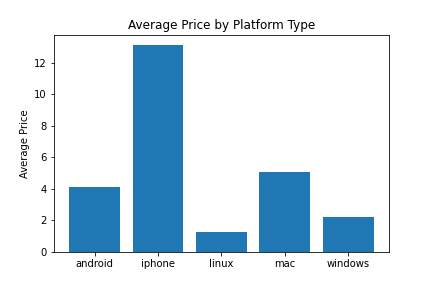
\includegraphics[scale=0.85]{img/Graphs/combinedData/priceHistogram_combinedData.png}
\centering
\caption{combinedData\_priceHistogram}
\label{fig:combinedData_priceHistogram}
\end{figure}

\subsection{Chat data}\label{EDA}

Chat data is a representation between messages send by the users. The EDA for this section wouldn't make much sense, therefore it was not completed. 

Reason why it doesn't make sense are attributes. Listed bellow are 6 attributes. This is all we have from the 4 files. 
\begin{itemize}
    \item userId
    \item teamchat\_session\_id
    \item date
    \item chat\_item
    \item chatid1
    \item chatid1
\end{itemize}

Out of 6 attributes, 5 of them are IDs and one of them is date. Time series analysis could be done for when messages were send, but that would be it. Since majority of items are IDs, this wouldn't add much of the business value. Regardless, we can see documented attributes for each of the files bellow.

\begin{center}
\begin{longtable}{ |l|l| } 
 \hline
 Attribute & Description\\ 
 \hline
 userId & ID of the user\\ 
 \hline
 teamchat\_session\_id & ID of the session that team is in\\ 
 \hline
 date & time of the operation\\ 
 \hline
\caption{chat\_join\_team\_chat.csv}
\end{longtable}
\end{center}

\begin{center}
\begin{longtable}{ |l|l| } 
 \hline
 Attribute & Description\\ 
 \hline
 userId & ID of the user\\ 
 \hline
 teamchat\_session\_id & ID of the session that team is in\\ 
 \hline
 date & time of the operation\\ 
 \hline
\caption{chat\_leave\_team\_chat.csv}
\end{longtable}
\end{center}

\begin{center}
\begin{longtable}{ |l|l| } 
 \hline
 Attribute & Description\\ 
 \hline
 chat\_item & ID of the message that was send\\ 
 \hline
 user\_id & ID of the user (that send the message)\\ 
 \hline
 date & time when message was send\\ 
 \hline
\caption{chat\_mention\_team\_chat.csv}
\end{longtable}
\end{center}

\begin{center}
\begin{longtable}{ |l|l| } 
 \hline
 Attribute & Description\\ 
 \hline
chatid1 & ID of the message that was send\\ 
 \hline
chatid2 & ID of the message that got responded\\ 
 \hline
 date & time when chatid2 was send\\ 
 \hline
\caption{chat\_respond\_team\_chat.csv}
\end{longtable}
\end{center}
\subsection{Flamingo data}\label{EDA}

\begin{center}
\begin{longtable}{ |l|l| } 
 \hline
 Attribute & Description\\ 
 \hline
 timestamp & when ad was clicked\\ 
 \hline
 txId & ID of the click\\ 
 \hline
 userSessionId & ID of the users session who made the click\\ 
 \hline
 teamId & ID of the team that user is in\\ 
 \hline
 userId & ID of the user that made the click\\ 
 \hline
 adId & ID of an add that was clicked\\ 
 \hline
 adCategory & type of an ad that was clicked\\ 
 \hline
\caption{ad-clicks.csv}
\end{longtable}
\end{center}

Inspecting for missing data in adClicks showcases no missing values.
\begin{figure}[H]
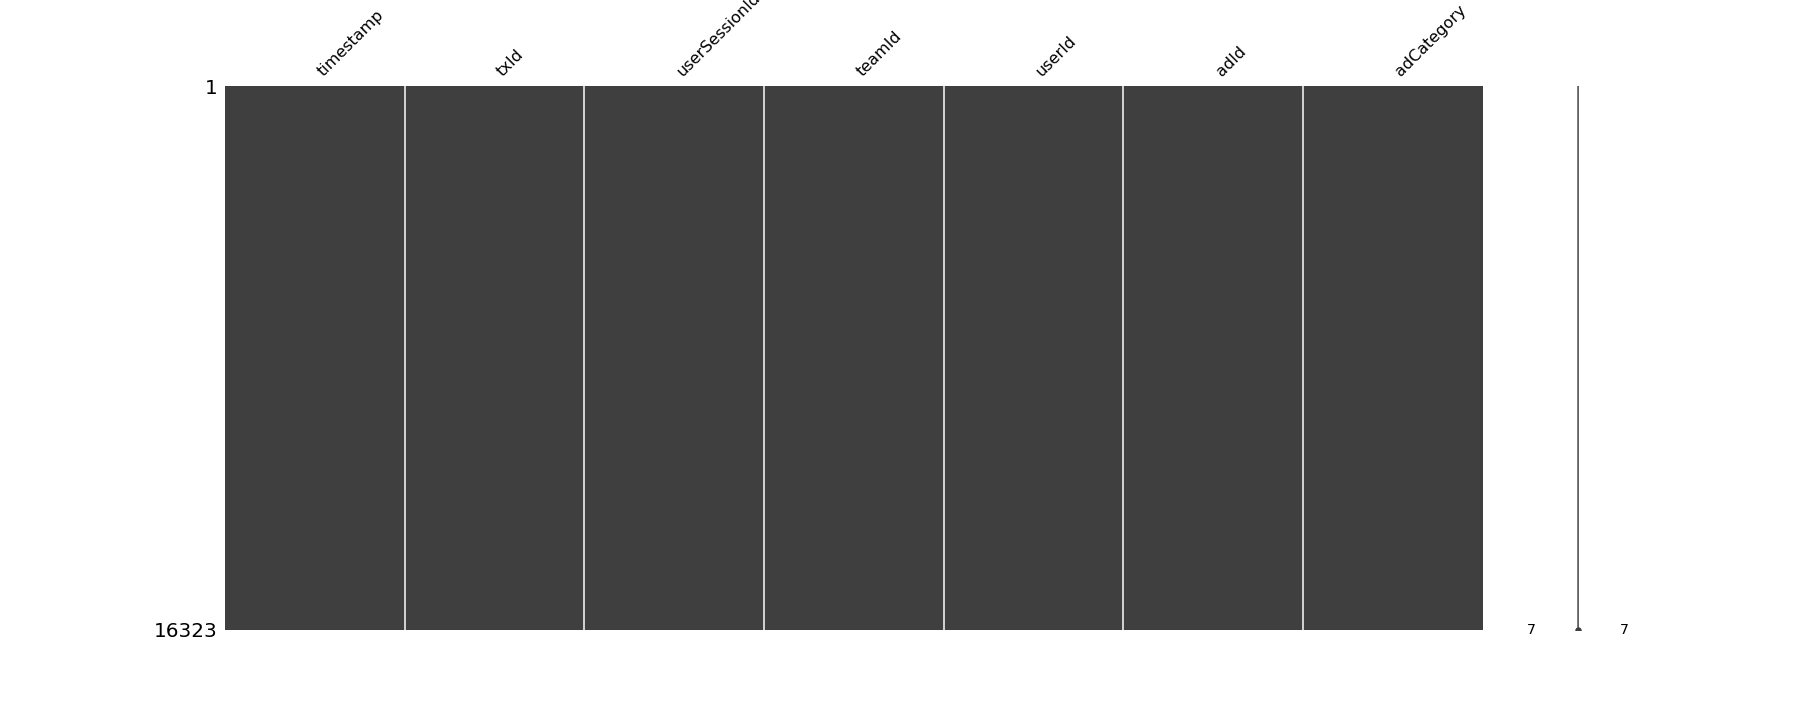
\includegraphics[scale=0.25]{img/Graphs/adClicks/missingno_adClicks.png}
\centering
\caption{adClicks\_msno}
\label{fig:adClicks_msno}
\end{figure}

Figure (ID) represents decline of ad clicks over time. From business point of view, decline looks steep and fast, therefore something must have happened with the game.
\begin{figure}[H]
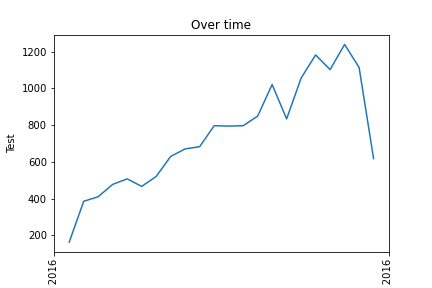
\includegraphics[scale=0.85]{img/Graphs/adClicks/timeseries_adClicks.png}
\centering
\caption{timeseries\_adClicks}
\label{fig:timeseries_adClicks}
\end{figure}

Looking at the biggest teams, we can see that team with id 64 has occurred 681 times. With knowing what top teams are doing, we can assume other teams will copy them.
\begin{figure}[H]
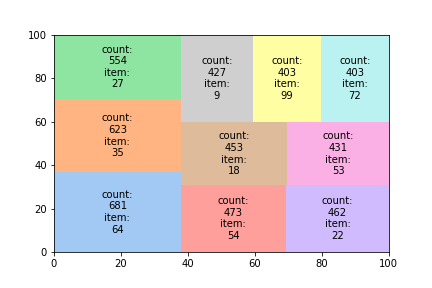
\includegraphics[scale=0.85]{img/Graphs/adClicks/tree_map_adClicks.png}
\centering
\caption{adClicks\_tree\_map}
\label{fig:adClicks_tree_map}
\end{figure}

Comparing IDs of ads to the sections they are representing, we can see that computers and games have the most IDs. This would make sense since the product we are offering is computer game. Other products have on average 3 IDs meaning they aren't so popular.
\begin{figure}[H]
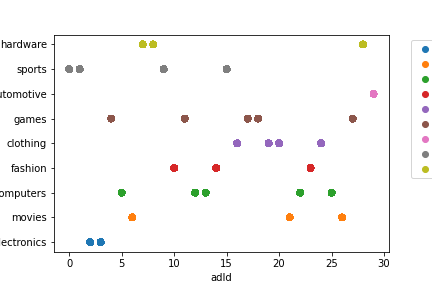
\includegraphics[scale=0.85]{img/Graphs/adClicks/create_ad_adClicks.png}
\centering
\caption{adClicks\_create\_ad}
\label{fig:adClicks_create_ad}
\end{figure}
\begin{center}
\begin{longtable}{ |l|l| } 
 \hline
 Attribute & Description\\ 
 \hline
 timestamp & when the purcahse was made\\ 
 \hline
 txId & ID of the purchase\\ 
 \hline
 userSessionId & ID of the user who made the purchase\\ 
 \hline
 team & is ID of the team that user is in\\ 
 \hline
 userId & is ID of the user that made the purchase\\ 
 \hline
 buyId & ID of purchased item\\ 
 \hline
 price & price of prucased item\\ 
 \hline
\caption{buy-clicks.csv}
\end{longtable}
\end{center}

Dataset buy-clicks appears to not have any missing data.
\begin{figure}[H]
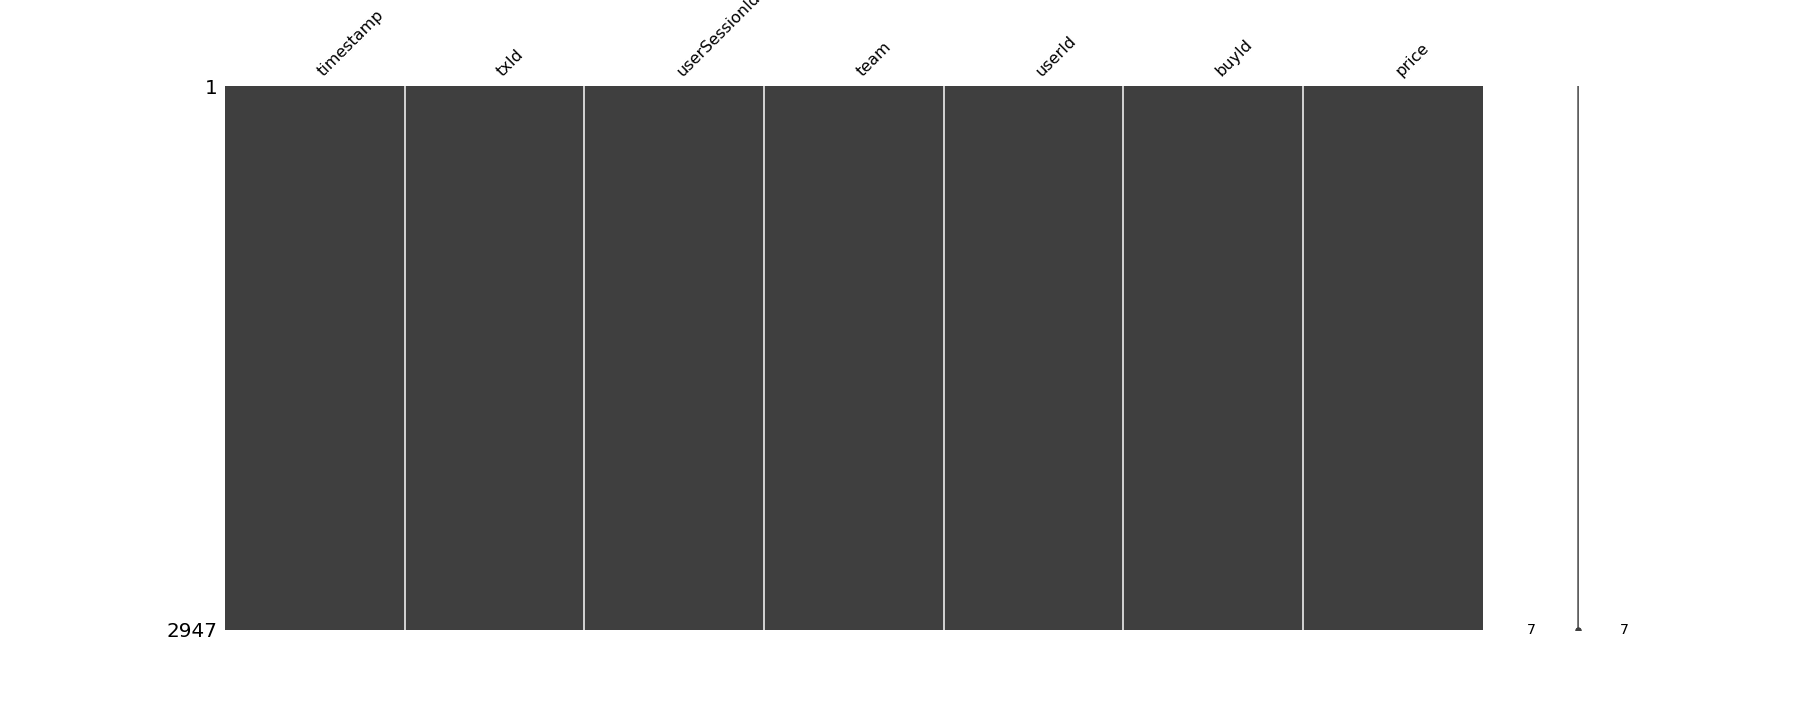
\includegraphics[scale=0.25]{img/Graphs/buyClicks/missingno_buyClicks.png}
\centering
\caption{missingno\_buyClicks}
\label{fig:missingno_buyClicks}
\end{figure}

Looking over the time series, graph is similar to ad-clicks in terms of decline. 
\begin{figure}[H]
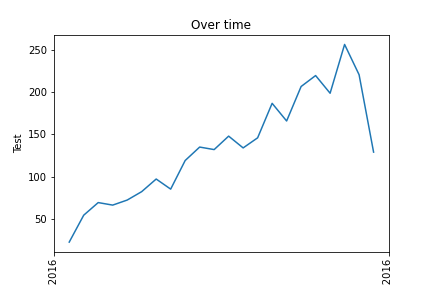
\includegraphics[scale=0.85]{img/Graphs/buyClicks/timeseries_buyClicks.png}
\centering
\caption{timeseries\_buyClicks}
\label{fig:timeseries_buyClicks}
\end{figure}

Investigating which team has bought the most items, we can see that team with id 27 is the top spender although it is only 3rd one in terms of team members. The second biggest spender, team 64, has the most members. This would put team 27 in odd position since they appear to be the perfect team (quite big and they spend the most).
\begin{figure}[H]
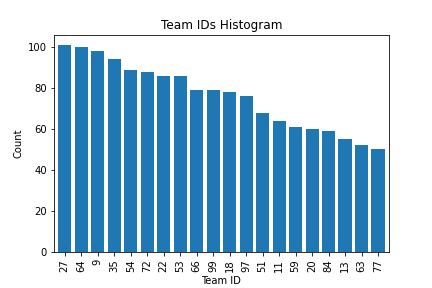
\includegraphics[scale=0.85]{img/Graphs/buyClicks/histogram_buyClicks.png}
\centering
\caption{histogram\_buyClicks}
\label{fig:histogram_buyClicks}
\end{figure}

Creating a correlation chart between team, price and buy ID shows us that team is not correlated to anything. On the other hand, buy id and price seems to be heavily correlated which we have confirmed with missing data in Combined data section (Figure \ref{fig:combinedData_msno}).
\begin{figure}[H]
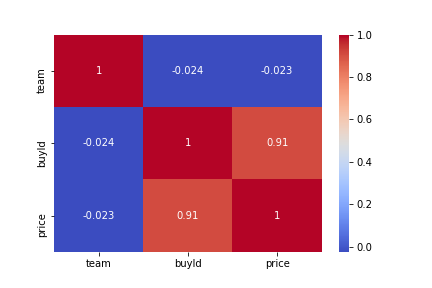
\includegraphics[scale=0.85]{img/Graphs/buyClicks/correlationPlot_buyClicks.png}
\centering
\caption{correlationPlot\_buyClicks}
\label{fig:correlationPlot_buyClicks}
\end{figure}
\begin{center}
\begin{longtable}{ |l|l| } 
 \hline
 Attribute & Description\\ 
 \hline
 timestamp & when click occurred\\ 
 \hline
 clickId & ID of the click\\ 
 \hline
 userId & ID of the user who clicked\\ 
 \hline
 userSessionId & ID of session that user was in\\ 
 \hline
 isHit & if flamingo was hit (1) or not (2)\\ 
 \hline
 teamId & ID of the team that user is in\\ 
 \hline
 teamLevel & level that team is in\\ 
 \hline
\caption{game-clicks.csv}
\end{longtable}
\end{center}

Game clicks doesn't appear to have any missing values.
\begin{figure}[H]
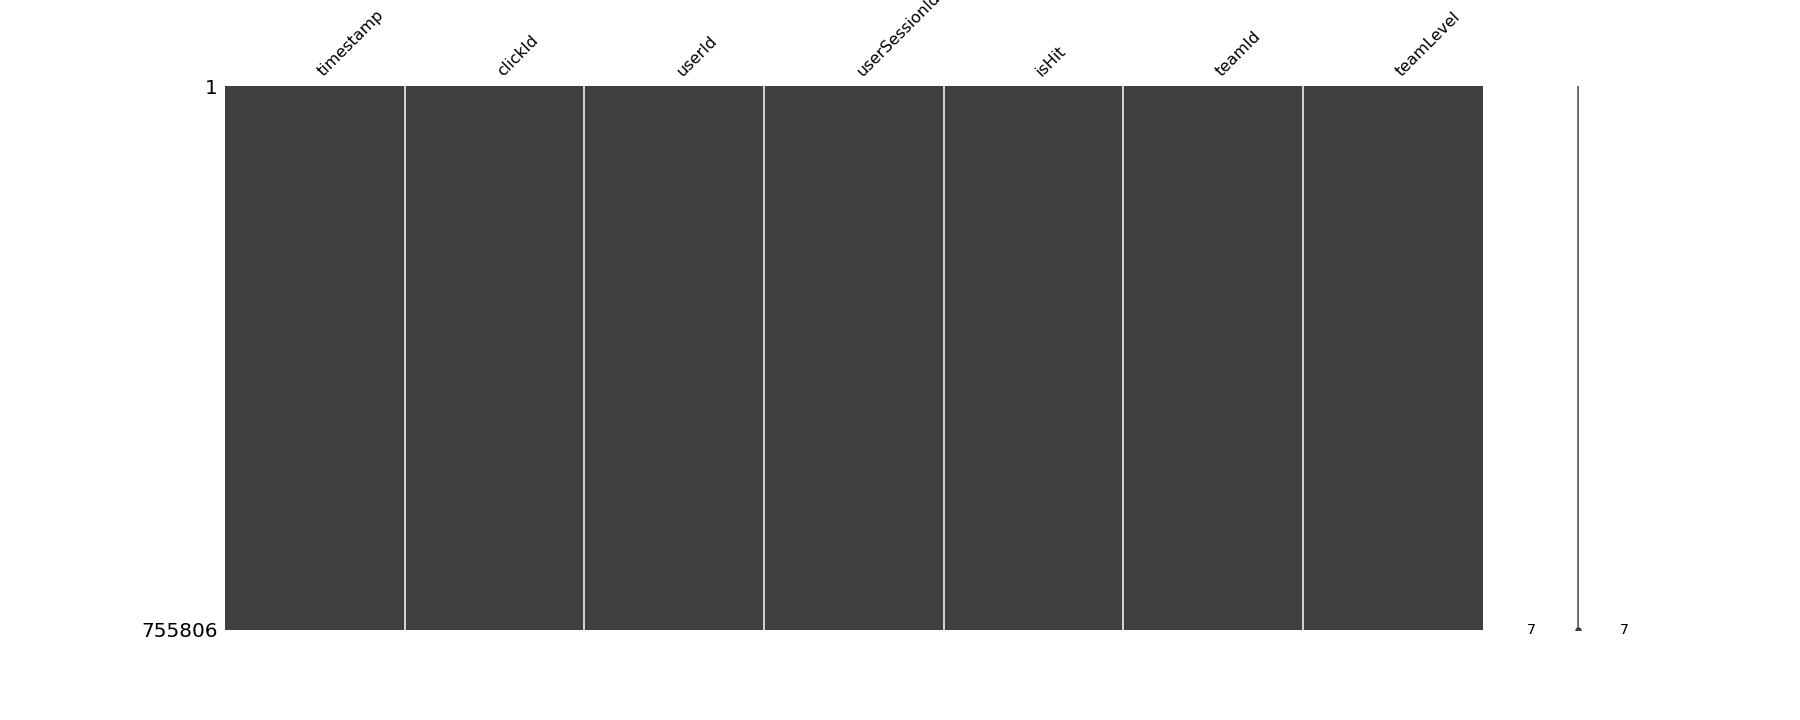
\includegraphics[scale=0.25]{img/Graphs/gameClicks/missingno_gameClicks.png}
\centering
\caption{missingno\_gameClicks}
\label{fig:missingno_gameClicks}
\end{figure}

Time series for game clicks again similar to previous graphs. The only difference is the line is much steeper.
\begin{figure}[H]
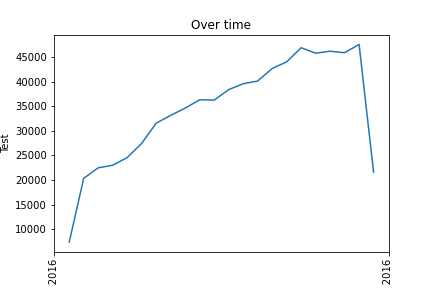
\includegraphics[scale=0.85]{img/Graphs/gameClicks/timeseries_gameClicks.png}
\centering
\caption{timeseries\_gameClicks}
\label{fig:timeseries_gameClicks}
\end{figure}
\begin{center}
\begin{longtable}{ |l|l| } 
 \hline
 Attribute & Description\\ 
 \hline
 timestamp & when the event occured\\ 
 \hline
 eventId & ID of the event\\ 
 \hline
 teamId & ID of the team\\ 
 \hline
 teamLevel & level that team has stared or completed\\ 
 \hline
 eventType & type of the event (start or end)\\ 
 \hline
\caption{level-events.csv}
\end{longtable}
\end{center}

Level events appears not to have any missing values.
\begin{figure}[H]
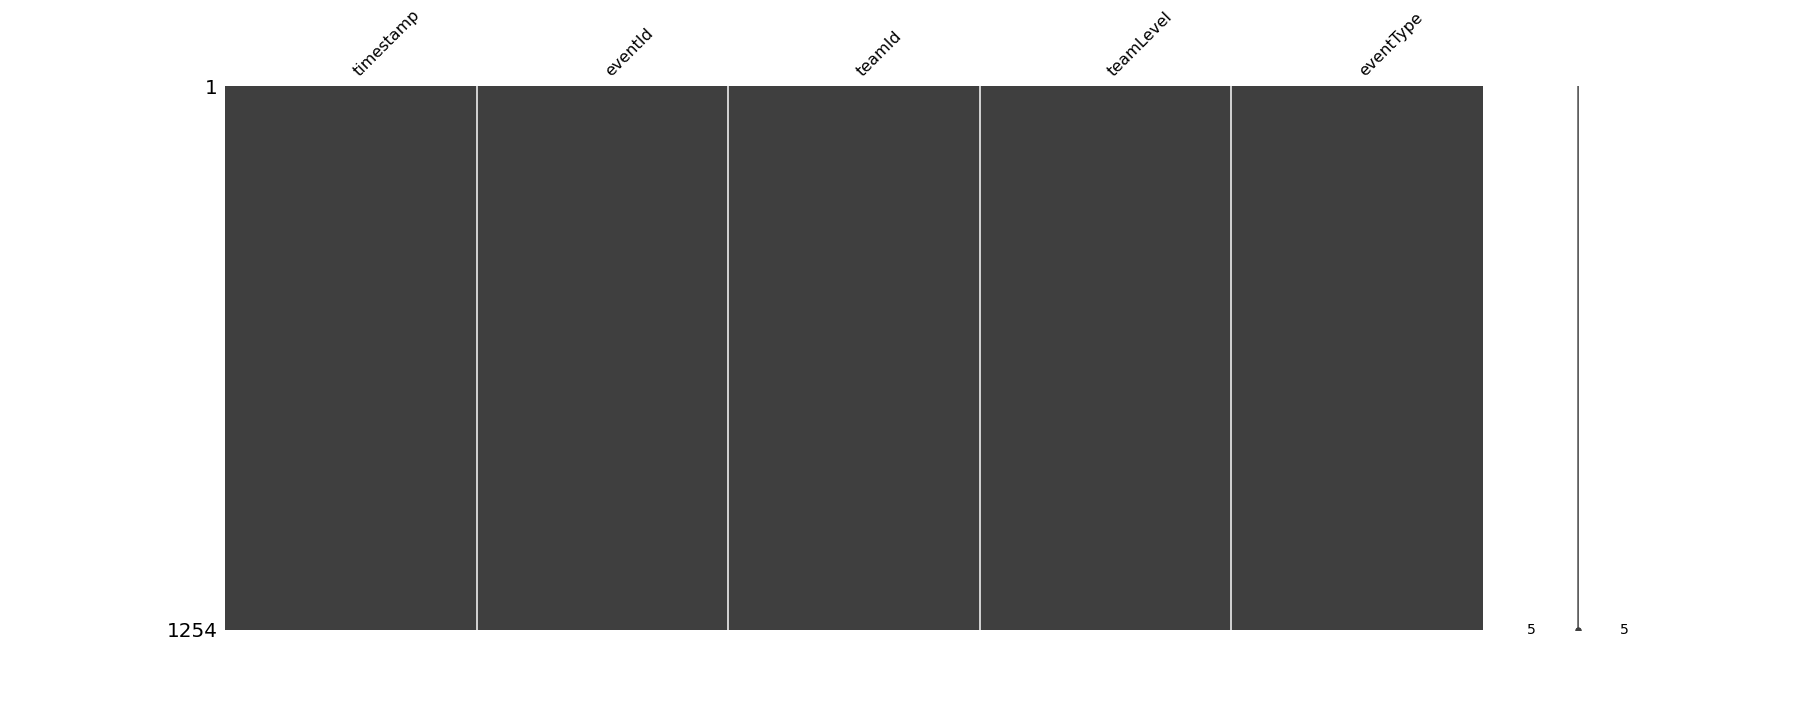
\includegraphics[scale=0.25]{img/Graphs/levelEvents/missingno_levelEvents.png}
\centering
\caption{missingno\_levelEvents}
\label{fig:missingno_levelEvents}
\end{figure}

The time series for level events is unusual. There appears to be 7 spikes, which could indicate when players went up the levels and then it finishing. Other possibility is game events occurring every so often. The graph itself does look different, but the ending seems to be the same as with other graphs. Analysing the graph left to right, we can see how it goes up and down. But at the end, it goes down from the spike, when we would expect it to go back up, it went down again. This seems to confirm that something odd has happened with time series so far.
\begin{figure}[H]
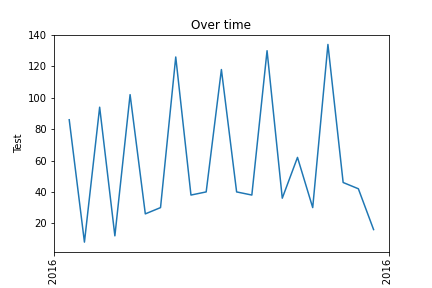
\includegraphics[scale=0.85]{img/Graphs/levelEvents/timeseries_levelEvents.png}
\centering
\caption{timeseries\_levelEvents}
\label{fig:timeseries_levelEvents}
\end{figure}
\begin{center}
\begin{longtable}{ |l|l| } 
 \hline
 Attribute & Description\\ 
 \hline
 timestamp & when the user joined the team\\ 
 \hline
 team & ID of the team\\ 
 \hline
 userId & ID of the user\\ 
 \hline
 assignmentId & Temp ID assigned to the user (while in the team/session)\\ 
 \hline
\caption{team-assignments.csv}
\end{longtable}
\end{center}

Team assignments dataframe has no missing data.
\begin{figure}[H]
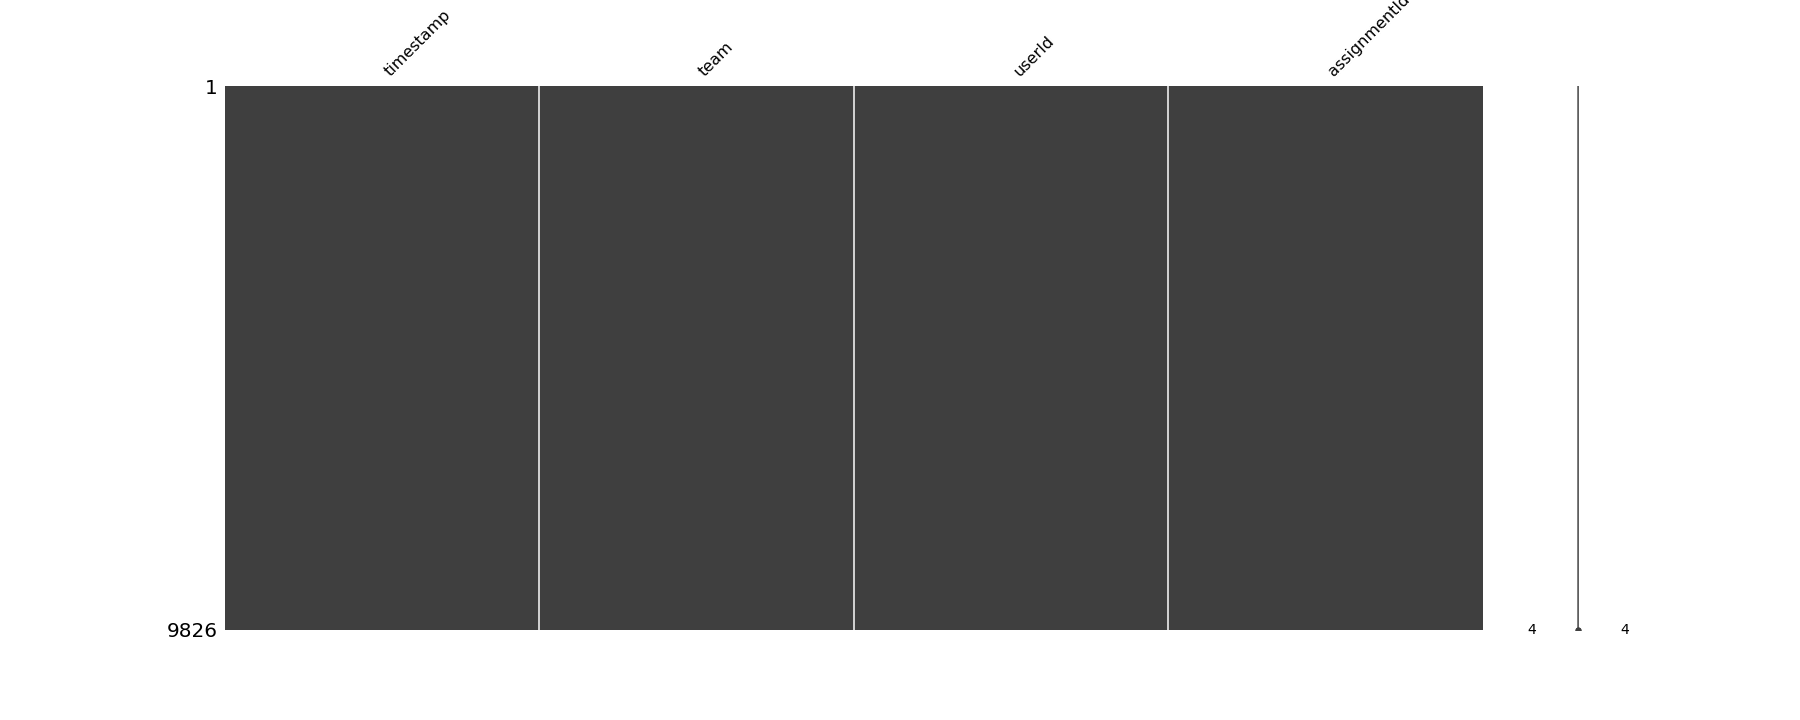
\includegraphics[scale=0.25]{img/Graphs/teamAssignments/missingno_teamAssignments.png}
\centering
\caption{missingno\_teamAssignments}
\label{fig:missingno_teamAssignments}
\end{figure}

At the beginning of the time series, we can see quite a steep decline. This was momental, since afterwards decline of team assignments is slow. At the end, we can observe a steep decline, that matches all the time sereies so far.
\begin{figure}[H]
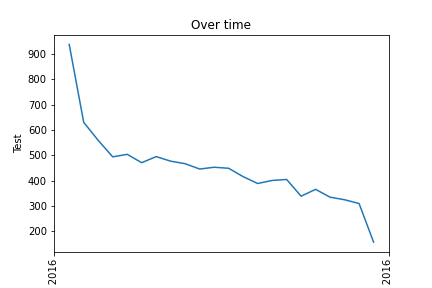
\includegraphics[scale=0.85]{img/Graphs/teamAssignments/timeseries_teamAssignments.png}
\centering
\caption{timeseries\_teamAssignments}
\label{fig:timeseries_teamAssignments}
\end{figure}
\begin{center}
\begin{longtable}{ |l|l| } 
 \hline
 Attribute & Description\\ 
 \hline
 teamId & ID of the team\\ 
 \hline
 name & name of the team\\ 
 \hline
 teamCreationTime & time when team was created\\ 
 \hline
 teamEndTime & time when last member left the team\\ 
 \hline
 strength & how strong the team is (based on performance)\\ 
 \hline
 currentLevel & current level of the team\\ 
 \hline
\caption{team.csv}
\end{longtable}
\end{center}

Team dataframe has no missing data.
\begin{figure}[H]
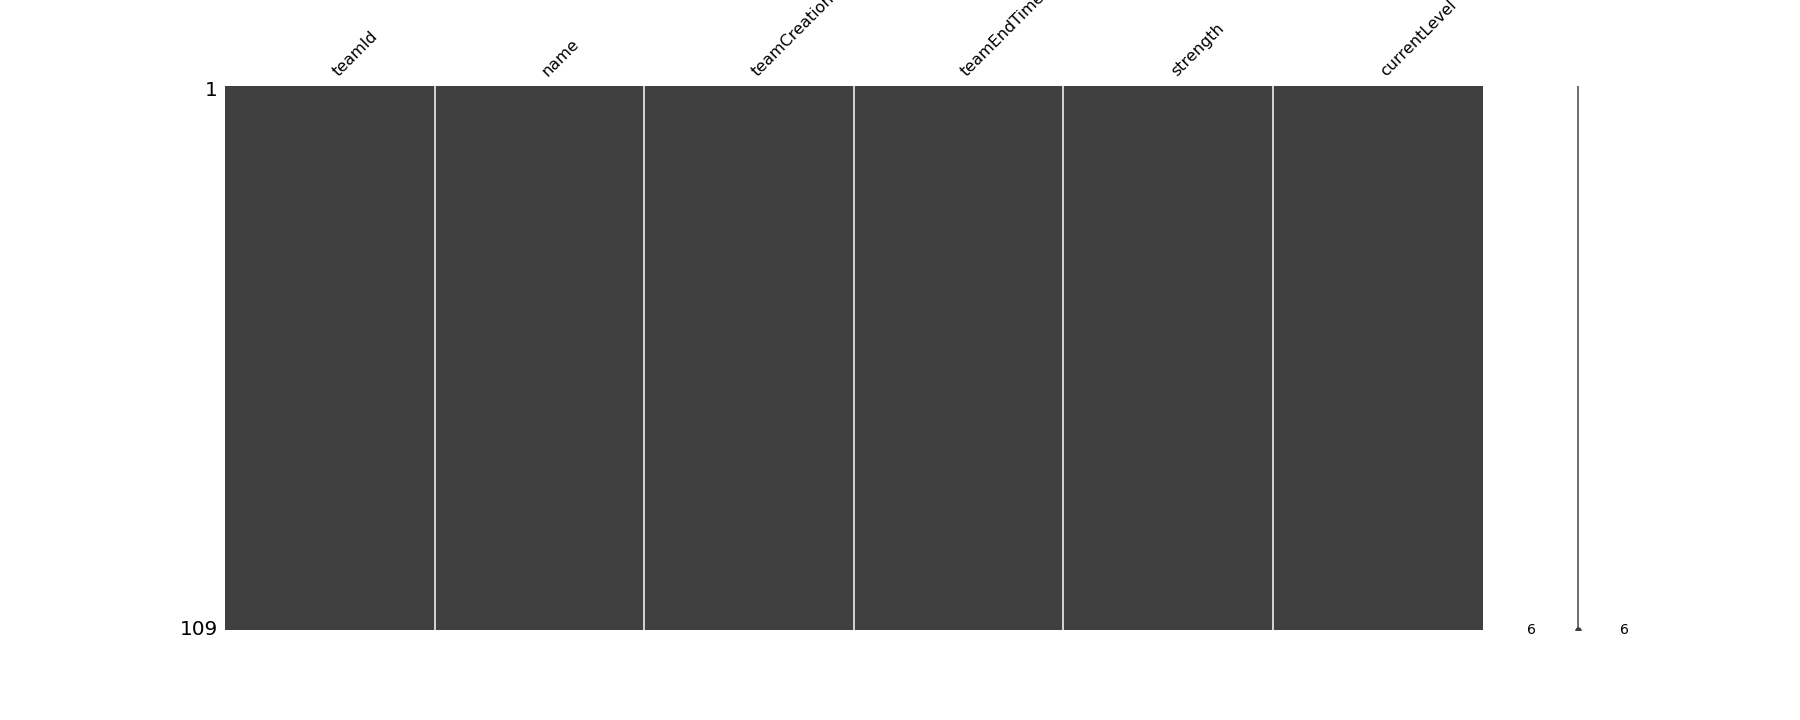
\includegraphics[scale=0.25]{img/Graphs/team/missingno_team.png}
\centering
\caption{missingno\_team}
\label{fig:missingno_team}
\end{figure}


% \begin{figure}[H]
% 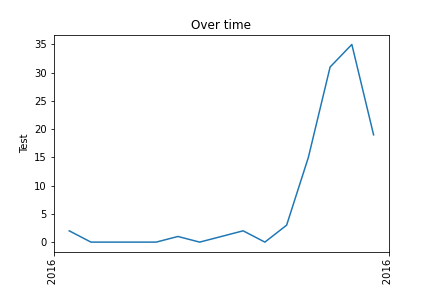
\includegraphics[scale=0.85]{img/Graphs/team/timeseries_team.png}
% \centering
% \caption{timeseries\_team}
% \label{fig:timeseries_team}
% \end{figure}

Analysing team creation time with team end time, we can see something odd. Blue line (representing team creation time) is showcasing how teams were created. Growth was slow, until it expend a lot. By that logic, there should be some teams that were ended (orange line). This can be seen from the start how teams were created and ended, but after a while there seems to be nothing regarding ending of the teams.

With this information, we can conclude two things:
\begin{itemize}
    \item As with time series from above, this one is effected as well,
    \item There seems to be missing data (as we have the data but it is wrong) for team end date since it straight up ends in the middle of the graph.
\end{itemize}
\begin{figure}[H]
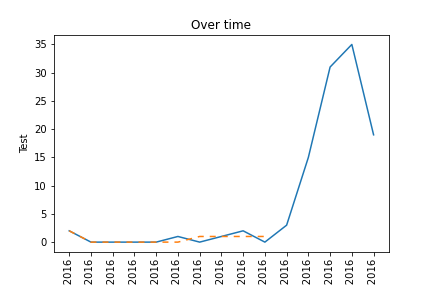
\includegraphics[scale=0.85]{img/Graphs/team/timeseries2_team.png}
\centering
\caption{timeseries2\_team}
\label{fig:timeseries2_team}
\end{figure}

The strongest teams on the graph do not appear on the list of the biggest teams. What is interesting is team with id 9, they are 3rd in terms of strength (Figure \ref{fig:teamStrength_team}) and in terms of spending ( Figure\ref{fig:histogram_buyClicks}). This team appears to spend the most and be the strongest at the same time being 4th biggest team in terms of members (Figure \ref{fig:adClicks_tree_map}).
\begin{figure}[H]
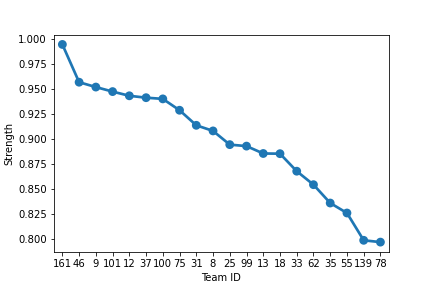
\includegraphics[scale=0.85]{img/Graphs/team/teamStrength_team.png}
\centering
\caption{teamStrength\_team}
\label{fig:teamStrength_team}
\end{figure}

Teams with lower strength do not appear in the biggest team section. But 4th weakest team appears to be on the lower section on spending.
\begin{figure}[H]
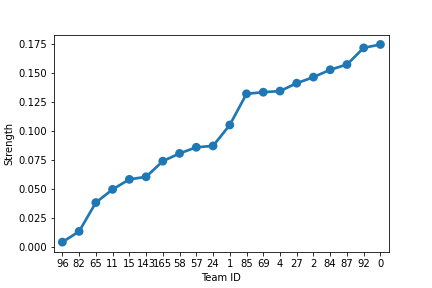
\includegraphics[scale=0.85]{img/Graphs/team/teamStrength2_team.png}
\centering
\caption{teamStrength2\_team}
\label{fig:teamStrength2_team}
\end{figure}
\begin{center}
\begin{longtable}{ |l|l| } 
 \hline
 Attribute & Description\\ 
 \hline
 timestamp & time when session started\\ 
 \hline
 userSessionId & ID of the session\\ 
 \hline
 userId & ID of the user in session\\ 
 \hline
 teamId & ID of the team that user is in\\ 
 \hline
 assignmentId & Temp ID assigned to the user (while in the team/session)\\ 
 \hline
 sessionType & type of the event (start or end)\\ 
 \hline
 teamLevel & level of the team in the current session\\ 
 \hline
 platformType & what device / platform is being used\\ 
 \hline
\caption{user-session.csv}
\end{longtable}
\end{center}

User session dataframe does not have any missing values.
\begin{figure}[H]
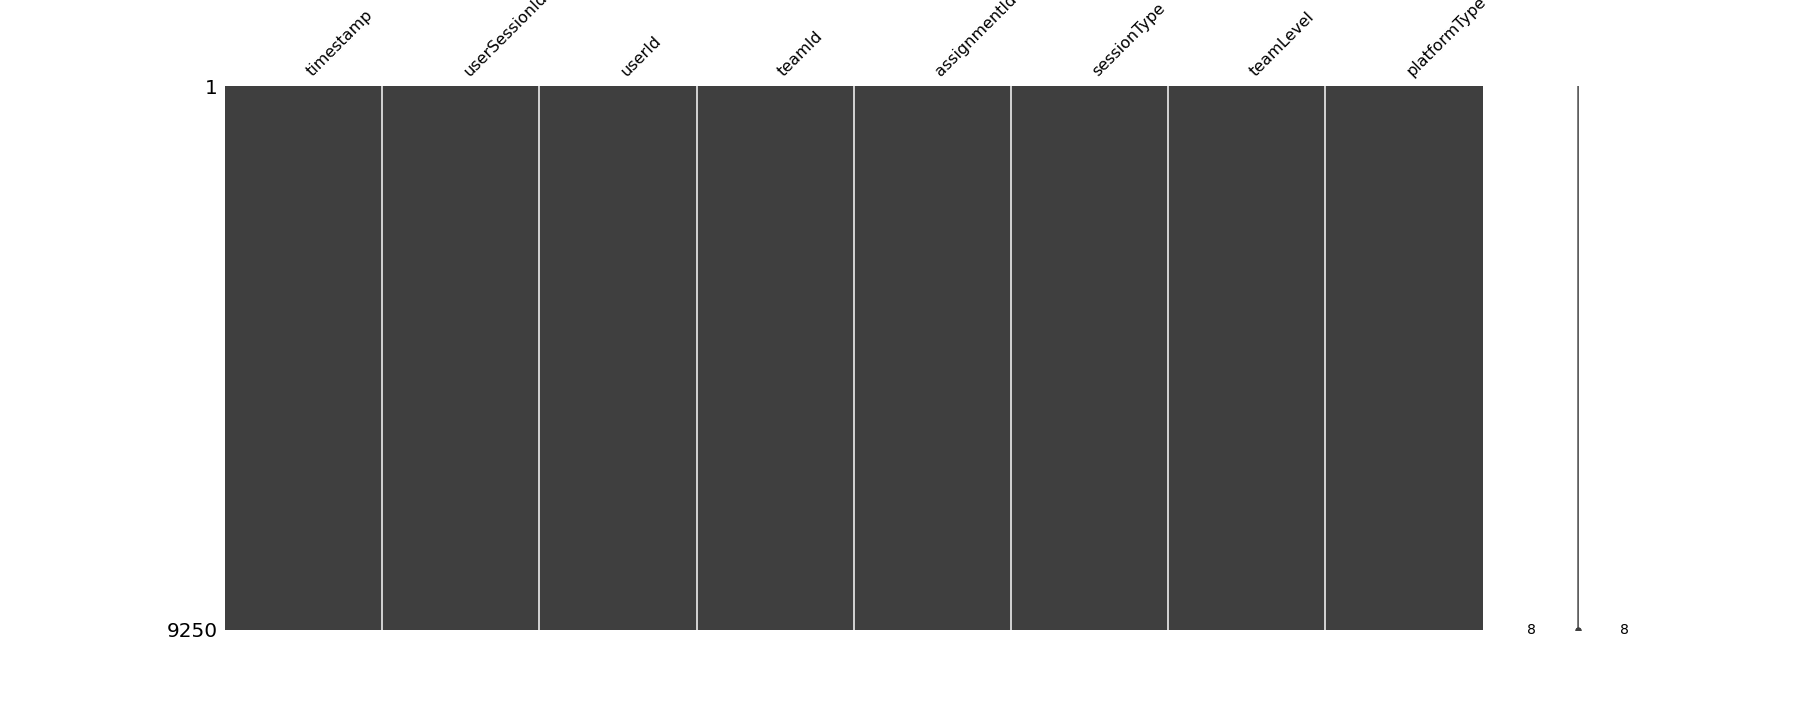
\includegraphics[scale=0.25]{img/Graphs/userSession/missingno_userSession.png}
\centering
\caption{missingno\_userSession}
\label{fig:missingno_userSession}
\end{figure}

Time series for user session appears to be spiky (simmilar to levelEvents, Figure \ref{fig:timeseries_levelEvents}). It ends with the same fall as other time series events.
\begin{figure}[H]
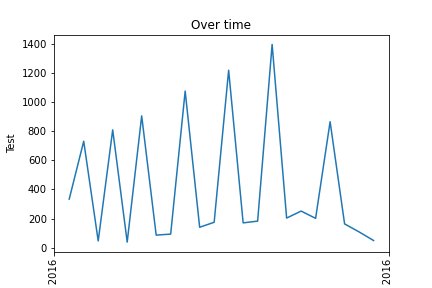
\includegraphics[scale=0.85]{img/Graphs/userSession/timeseries_userSession.png}
\centering
\caption{timeseries\_userSession}
\label{fig:timeseries_userSession}
\end{figure}

If we compare start and end of sessions for platforms, we can see that users tend not to switch platforms while the session is running. This could be one of the game limitations, meaning if you would rejoin from other platform, your session would expire.
\begin{figure}[H]
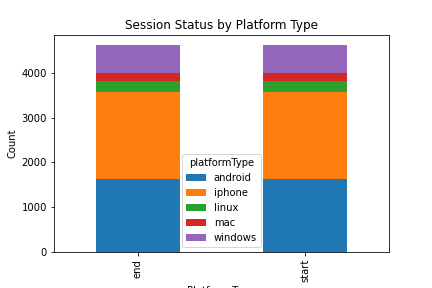
\includegraphics[scale=0.85]{img/Graphs/userSession/histogram_userSession.png}
\centering
\caption{histogram\_userSession}
\label{fig:histogram_userSession}
\end{figure}
\begin{center}
\begin{longtable}{ |l|l| } 
 \hline
 Attribute & Description\\ 
 \hline
 timestamp & time when first game starts\\ 
 \hline
 userId & ID of the user\\ 
 \hline
 nick & nickname chosen by the user\\ 
 \hline
 twitter & twitter handle of the user\\ 
 \hline
 dob & date of birth of the user\\ 
 \hline
 country & two letter country code of the user\\ 
 \hline
\caption{user.csv}
\end{longtable}
\end{center}

Data frame users is the first one (in this path) to have missing data. The data that is missing is in country and it is a small amount.
\begin{figure}[H]
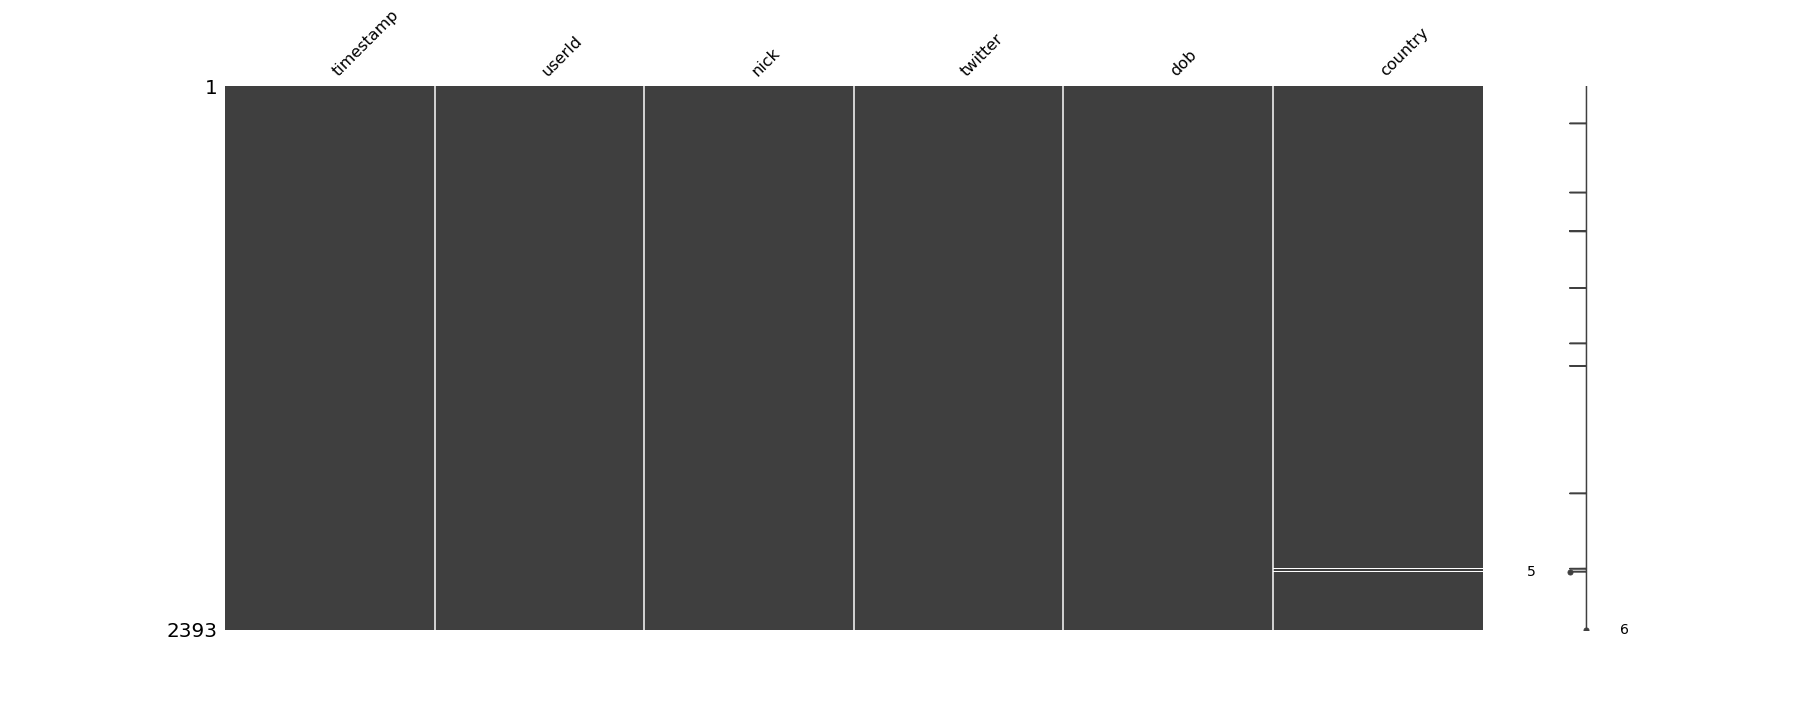
\includegraphics[scale=0.25]{img/Graphs/users/missingno_user.png}
\centering
\caption{missingno\_users}
\label{fig:missingno_user}
\end{figure}

The demographic of our users seem to be on the younger side. The majority of players seem to be born after 1970.
\begin{figure}[H]
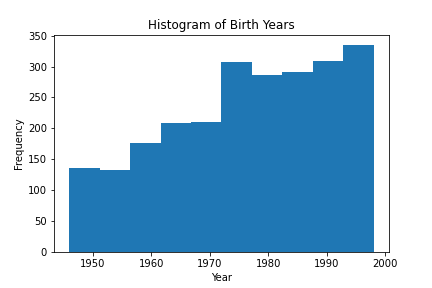
\includegraphics[scale=0.85]{img/Graphs/users/histogram_users.png}
\centering
\caption{histogram\_userSession}
\label{fig:histogram_users}
\end{figure}

\begin{landscape}
Geographically looking there seems to be players from all around the globe. This is good in terms of different markets and bad in terms of computational overhead (since we need computers in all of the regions for optimal performance).

    \begin{figure}[H]
        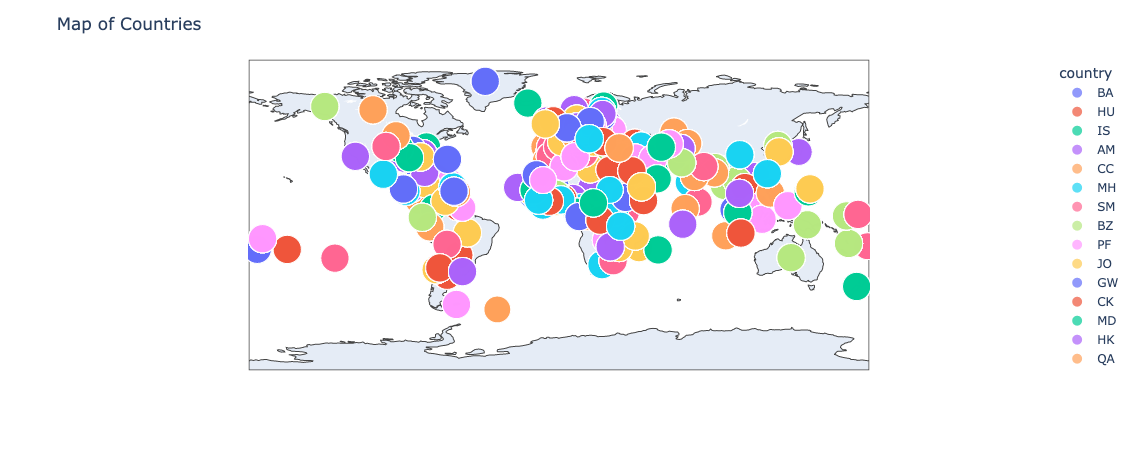
\includegraphics[scale=0.65]{img/Graphs/users/map.png}
        \centering
        \caption{map}
        \label{fig:map}
    \end{figure}
\end{landscape}
